\documentclass[symmetric,justified,marginals=raggedouter]{tufte-book}

%\hypersetup{colorlinks}% uncomment this line if you prefer colored hyperlinks (e.g., for onscreen viewing)

%%
% If they're installed, use Bergamo and Chantilly from www.fontsite.com.
% They're clones of Bembo and Gill Sans, respectively.
%\IfFileExists{bergamo.sty}{\usepackage[osf]{bergamo}}{}% Bembo
%\IfFileExists{chantill.sty}{\usepackage{chantill}}{}% Gill Sans

%\usepackage{microtype}

%%
% For nicely typeset tabular material
\usepackage{booktabs}

%%
% For graphics / images
\usepackage{graphicx}
\setkeys{Gin}{width=\linewidth,totalheight=\textheight,keepaspectratio}
\graphicspath{{graphics/}}

% The fancyvrb package lets us customize the formatting of verbatim
% environments.  We use a slightly smaller font.
\usepackage{fancyvrb}
\fvset{fontsize=\normalsize}

%%
% Prints argument within hanging parentheses (i.e., parentheses that take
% up no horizontal space).  Useful in tabular environments.
\newcommand{\hangp}[1]{\makebox[0pt][r]{(}#1\makebox[0pt][l]{)}}

%%
% Prints an asterisk that takes up no horizontal space.
% Useful in tabular environments.
\newcommand{\hangstar}{\makebox[0pt][l]{*}}

%%
% Prints a trailing space in a smart way.
\usepackage{xspace}

%%
% Some shortcuts for Tufte's book titles.  The lowercase commands will
% produce the initials of the book title in italics.  The all-caps commands
% will print out the full title of the book in italics.
\newcommand{\vdqi}{\textit{VDQI}\xspace}
\newcommand{\ei}{\textit{EI}\xspace}
\newcommand{\ve}{\textit{VE}\xspace}
\newcommand{\be}{\textit{BE}\xspace}
\newcommand{\VDQI}{\textit{The Visual Display of Quantitative Information}\xspace}
\newcommand{\EI}{\textit{Envisioning Information}\xspace}
\newcommand{\VE}{\textit{Visual Explanations}\xspace}
\newcommand{\BE}{\textit{Beautiful Evidence}\xspace}

\newcommand{\TL}{Tufte-\LaTeX\xspace}

% Prints the month name (e.g., January) and the year (e.g., 2008)
\newcommand{\monthyear}{%
  \ifcase\month\or January\or February\or March\or April\or May\or June\or
  July\or August\or September\or October\or November\or
  December\fi\space\number\year
}


% Prints an epigraph and speaker in sans serif, all-caps type.
\newcommand{\openepigraph}[2]{%
  %\sffamily\fontsize{14}{16}\selectfont
  \begin{fullwidth}
  \sffamily\large
  \begin{doublespace}
  \noindent\allcaps{#1}\\% epigraph
  \noindent\allcaps{#2}% author
  \end{doublespace}
  \end{fullwidth}
}

% Inserts a blank page
\newcommand{\blankpage}{\newpage\hbox{}\thispagestyle{empty}\newpage}

\usepackage{units}

% Typesets the font size, leading, and measure in the form of 10/12x26 pc.
\newcommand{\measure}[3]{#1/#2$\times$\unit[#3]{pc}}

% Macros for typesetting the documentation
\newcommand{\hlred}[1]{\textcolor{Maroon}{#1}}% prints in red
\newcommand{\hangleft}[1]{\makebox[0pt][r]{#1}}
\newcommand{\hairsp}{\hspace{1pt}}% hair space
\newcommand{\hquad}{\hskip0.5em\relax}% half quad space
\newcommand{\TODO}{\textcolor{red}{\bf TODO!}\xspace}
\newcommand{\ie}{\textit{i.\hairsp{}e.}\xspace}
\newcommand{\eg}{\textit{e.\hairsp{}g.}\xspace}
\newcommand{\na}{\quad--}% used in tables for N/A cells
\providecommand{\XeLaTeX}{X\lower.5ex\hbox{\kern-0.15em\reflectbox{E}}\kern-0.1em\LaTeX}
\newcommand{\tXeLaTeX}{\XeLaTeX\index{XeLaTeX@\protect\XeLaTeX}}
% \index{\texttt{\textbackslash xyz}@\hangleft{\texttt{\textbackslash}}\texttt{xyz}}
\newcommand{\tuftebs}{\symbol{'134}}% a backslash in tt type in OT1/T1
\newcommand{\doccmdnoindex}[2][]{\texttt{\tuftebs#2}}% command name -- adds backslash automatically (and doesn't add cmd to the index)
\newcommand{\doccmddef}[2][]{%
  \hlred{\texttt{\tuftebs#2}}\label{cmd:#2}%
  \ifthenelse{\isempty{#1}}%
    {% add the command to the index
      \index{#2 command@\protect\hangleft{\texttt{\tuftebs}}\texttt{#2}}% command name
    }%
    {% add the command and package to the index
      \index{#2 command@\protect\hangleft{\texttt{\tuftebs}}\texttt{#2} (\texttt{#1} package)}% command name
      \index{#1 package@\texttt{#1} package}\index{packages!#1@\texttt{#1}}% package name
    }%
}% command name -- adds backslash automatically
\newcommand{\doccmd}[2][]{%
  \texttt{\tuftebs#2}%
  \ifthenelse{\isempty{#1}}%
    {% add the command to the index
      \index{#2 command@\protect\hangleft{\texttt{\tuftebs}}\texttt{#2}}% command name
    }%
    {% add the command and package to the index
      \index{#2 command@\protect\hangleft{\texttt{\tuftebs}}\texttt{#2} (\texttt{#1} package)}% command name
      \index{#1 package@\texttt{#1} package}\index{packages!#1@\texttt{#1}}% package name
    }%
}% command name -- adds backslash automatically
\newcommand{\docopt}[1]{\ensuremath{\langle}\textrm{\textit{#1}}\ensuremath{\rangle}}% optional command argument
\newcommand{\docarg}[1]{\textrm{\textit{#1}}}% (required) command argument
\newenvironment{docspec}{\begin{quotation}\ttfamily\parskip0pt\parindent0pt\ignorespaces}{\end{quotation}}% command specification environment
\newcommand{\docenv}[1]{\texttt{#1}\index{#1 environment@\texttt{#1} environment}\index{environments!#1@\texttt{#1}}}% environment name
\newcommand{\docenvdef}[1]{\hlred{\texttt{#1}}\label{env:#1}\index{#1 environment@\texttt{#1} environment}\index{environments!#1@\texttt{#1}}}% environment name
\newcommand{\docpkg}[1]{\texttt{#1}\index{#1 package@\texttt{#1} package}\index{packages!#1@\texttt{#1}}}% package name
\newcommand{\doccls}[1]{\texttt{#1}}% document class name
\newcommand{\docclsopt}[1]{\texttt{#1}\index{#1 class option@\texttt{#1} class option}\index{class options!#1@\texttt{#1}}}% document class option name
\newcommand{\docclsoptdef}[1]{\hlred{\texttt{#1}}\label{clsopt:#1}\index{#1 class option@\texttt{#1} class option}\index{class options!#1@\texttt{#1}}}% document class option name defined
\newcommand{\docmsg}[2]{\bigskip\begin{fullwidth}\noindent\ttfamily#1\end{fullwidth}\medskip\par\noindent#2}
\newcommand{\docfilehook}[2]{\texttt{#1}\index{file hooks!#2}\index{#1@\texttt{#1}}}
\newcommand{\doccounter}[1]{\texttt{#1}\index{#1 counter@\texttt{#1} counter}}

% Generates the index
\usepackage{makeidx}
\makeindex


\usepackage{indentfirst}

\usepackage[utf8]{inputenc}
\usepackage[T1]{fontenc}

%%%%%%%%%%%%%%%%%%%%%%%%%%%%%%%% Customization %%%%%%%%%%%%%%%%%%%%%%%%%%%%%%%%

\setcounter{tocdepth}{1}
\setcounter{secnumdepth}{1}

\renewcommand\contentsname{\normalfont \huge Table des matières}

\titlecontents{chapter}%
    [0em]% distance from left margin
    {\vspace{1\baselineskip}\begin{fullwidth}Chapitre }% above (global formatting of entry)
    {\contentslabel{0em} \hspace{1em} \huge $\vert$ \Large}% before w/ label (label = ``Chapter 1'')
    {\hspace{1em}}% before w/o label
    {\hfill\qquad\thecontentspage}% filler and page (leaders and page num)
    [\end{fullwidth}]% after
\titlecontents{section}% FIXME
    [0em] % distance from left margin
    {\vspace{0\baselineskip}\begin{fullwidth} \rmfamily\itshape} % above (global formatting of entry)
    {\hspace*{6em}\contentslabel{2em}} % before w/label (label = ``2.6'')
    {\hspace*{7em}} % before w/o label
    {\normalfont\hfill\qquad\thecontentspage} % filler + page (leaders and page num)
    [\end{fullwidth}] % after

\usepackage{enumitem}
\setlist{leftmargin=20mm}

\usepackage{tikz}
\usetikzlibrary{calc}

\newcommand\tikzmark[1]{%
  \tikz[overlay,remember picture] \coordinate (#1);}

\begin{document}

% Front matter
\frontmatter

%%%%%%%%%%%%%%%%%%%%%%%%%%%%%%%%%%%% Titre %%%%%%%%%%%%%%%%%%%%%%%%%%%%%%%%%%%%

\newpage
\author{Quentin Lobbé}
\title{\nohyphenation{Archives et Fragments Web}}
\cleardoublepage
{  
  \begin{fullwidth}%
  \thispagestyle{empty} 
  \setlength{\parskip}{\baselineskip}
  \begingroup
  \vspace*{10em}
  \par\noindent\Large{Quentin Lobbé}
  \vspace*{-1em}
  \par\noindent\Huge\textbf{Archives et Fragments Web}
  \par\noindent\nohyphenation\Large{Désagréger les archives Web pour mener une exploration temporelle de traces numériques des migrations}
  \endgroup
  \vfill  
  \par\noindent\nohyphenation Université Paris-Saclay, École doctorale des sciences et technologies de l'information et de la communication.  Thèse pour l'obtention du doctorat de Télécom ParisTech et de l'Université Paris-Saclay.    
  \end{fullwidth}%
}

\blankpage

%%%%%%%%%%%%%%%%%%%%%%%%%%%%%%%%%%%% Info Thèse %%%%%%%%%%%%%%%%%%%%%%%%%%%%%%%%%%%%
  
\newpage
\begin{fullwidth}
~\vfill
\thispagestyle{empty}
\setlength{\parskip}{\baselineskip}

\par\noindent Thèse présentée par \textbf{\thanklessauthor}\\
LTCI, Télécom ParisTech, Université Paris Saclay \& Inria. Paris, France.\\
quentin.lobbe@telecom-paristech.fr

\par\noindent Sous la direction de :\\
\textbf{Pierre Senellart}, professeur à l'École Normale Supérieure\\
\textbf{Dana Diminescu}, professeure à Télécom ParisTech

\par\noindent Soutenue publiquement à Paris le 9 novembre 2018, devant un jury composé de :\\
\textbf{Bruno Bachimont} (Rapporteur), enseignant-chercheur à l'Université Technologique de Compiègne\\
\textbf{Marc Spaniol} (Rapporteur), professeur à l'Université de Caen Basse-Normandie\\
\textbf{Anat Ben-David}, professeure à l'Open University of Israel\\
\textbf{Dominique Cardon}, professeur associé à Sciences Po Paris\\
\textbf{Bruno Defude}, directeur adjoint de la recherche et des formations doctorales à Télécom SudParis

\par\textit{last modified \monthyear}
\end{fullwidth}
  
\thispagestyle{empty}%
\clearpage%

%%%%%%%%%%%%%%%%%%%%%%%%%%%%%%%% Remerciements %%%%%%%%%%%%%%%%%%%%%%%%%%%%%%%%

\newpage

~\vfill
\noindent
\par\noindent Il me demanda de chercher la première page.\\
\noindent Je posais ma main gauche sur la couverture et ouvris le volume de mon pouce serré contre l'index. Je m'efforçais en vain : il restait toujours des feuilles entre la couverture et mon pouce. Elles semblaient sourdre du livre.\\
- Maintenant cherchez la dernière.\\
\noindent Mes tentatives échouèrent de même; à peine pus-je balbutier d'une voix qui n'était plus ma voix :\\
- Cela n'est pas possible.\\
\noindent Toujours à voix basse le vendeur me dit : \\
- Cela n'est pas possible et pourtant cela \textit{est}. Le nombre de pages de ce livre est exactement infini. Aucune n'est la première, aucune n'est la dernière.
\\~\\
\noindent\textit{Jorge Luis Borges - Le livre de sable} 
\vfill
\indent
\newpage
\begingroup
\vspace*{8em}
\huge $\vert$ \huge Remerciements
\vspace*{4em}
\par\normalsize Ici je remercie plein de gens

\par Beaucoup de gens

\par Mais vraiment
\endgroup
\vfill

%%%%%%%%%%%%%%%%%%%%%%%%%%%%%%%%%%%% Tables %%%%%%%%%%%%%%%%%%%%%%%%%%%%%%%%%%%%

\tableofcontents

\listoffigures

\listoftables

\mainmatter

%%%%%%%%%%%%%%%%%%%%%%%%%%%%%%%%%% Chapitre 1 %%%%%%%%%%%%%%%%%%%%%%%%%%%%%%%%%%

\chapter{Introduction}

\section{Introduction générale}

Ici l'intro de la thèse.

\section{Mise en garde}

\subsection{Penser le passé depuis le présent}

Ici on fait un rapide détour par l'historiographie et les difficultés à parler du passé depuis le présent.

\subsection{Conservation différentielle et nature des archives Web}

Ici on parle de la raréfaction de la matière Web à mesure que l'on remonte le temps et également à mesure que le web fournit du contenu.

%%%%%%%%%%%%%%%%%%%%%%%%%%%%%%%%%% Chapitre 2 %%%%%%%%%%%%%%%%%%%%%%%%%%%%%%%%%%

\chapter{Du Web aux Représentations en Ligne des Diasporas}
\label{chap:2}

\section{Retour aux origines du Web}

\section{Le migrant connecté}

\section{Le Web, espace de communication et d'organisation}

The Web is the main publishing application of the Internet.
As such, it consists mainly of the combination of three standards, the URI (Berners-Lee 1994) defining a naming space for object on the Internet, 6 HTTP (Fielding et al. 1999) defining a client–server interaction protocol using hyperlinks at its core, and HTML (Berners-Lee and Connolly 1995) an SGML DTD that defines the layout rendering of pages in browsers.
The implementation of these three standards enables any computer connected to the Internet to be- come a publishing system.

But the fact that it is actionable on the Web changes the way references are used by fragmenting content to smaller addressable pieces and overall favoring transversal navigation and access to content which in return, deeply changes the nature of writing as well as reading (Aarseth 1997; Landow 1997; Bolter 2001).

Géopolitique de l'hypertexte

Le web est un digital cultural artifact (Lyman and Kahle 1998)

 the Web does, to a large extend, re-use previous forms of publishing 12 (Crowston and Williams 1997; Eriksen and Ihlström 2000; Shepherd and Polanyi 2000), it also invents new ones.
 
This characterization of the Web as a distributed hypermedia openly and permanently authored at a global scale entails that Web archiving can only achieve preservation of limited aspects of a larger and living cultural artifact.

the interconnectedness of content is a major quality of the Web that raises issues when it comes to archiving.

\section{L'Atlas e-Diasporas}
\label{sec:2_atlas}

%%%%%%%%%%%%%%%%%%%%%%%%%%%%%%%%%% Chapitre 3 %%%%%%%%%%%%%%%%%%%%%%%%%%%%%%%%%%

\chapter{Préserver l'héritage numérique}

\noindent Face à la disparition totale ou partielle des sites Web recensés par l'atlas e-Diasporas (Chapitre \ref{chap:2}), il a été décidé de lancer une campagne d'archivage afin de préserver cet héritage numérique et d'anticiper, par là même, la tenue de futures recherches. Sans cette initiative, mes travaux de thèse n'auraient pas pu exploiter et questionner les traces d'un Web aujourd'hui passé. 

De part la nature même du médium, le Web demande de penser et de mettre en place un archivage particulier, basé sur des techniques de collectage dédiées. Dans ce chapitre, nous évoquerons la genèse de l'archivage du Web qui, au tournant des années 2000, a connu un essor mondial, mobilisant nombre d'acteurs et d'institutions. Nous introduirons ensuite, d'un point de vue technique, les principales méthodes de sélection, collecte et stockage des corpus à archiver. Nous présenterons enfin les contours des archives e-Diasporas à proprement parler. Ses particularités et ses caractéristiques. Sa durée et son étendue. \\

\noindent Bien que cette thèse se concentre sur l'exploration d'archives Web déjà existantes, il nous semble important d'évoquer la façon dont ces dernières sont constituées en amont afin de mieux saisir les biais analytiques (Chapitre \ref{chap:4}) qui motiveront la présentation de notre principale contribution (Chapitre \ref{chap:5}). Ce faisant, les éléments que nous nous apprêtons à présenter s'appuieront principalement sur l'ouvrage de J.~Masanes : "\textit{Web Archiving}" \citep{masanes_web_2006} qui reste encore aujourd'hui une référence.

\section{Vingt ans d'archivage du Web}

\noindent En Octobre 2016, se tenait à la Bibliothèque Nationale de France (BNF) une grande conférence anniversaire réunissant, pour les 20 ans de l'archivage du Web\footnote{\url{http://www.bnf.fr/fr/professionnels/anx_journees_pro_2016/a.jp_161122_23_archivage_web.html}}, les acteurs français de la pratique. Alors qu'était évoqués les conditions du partage du dépôt légal du Web national entre la BNF et l'INA, il a été rappelé qu'à l'origine chacune des deux institutions souhaitait se voir attribuer la pleine gestion de ce dépôt. L'INA mettait en avant ses compétences technique quant à l'archivage d'objets nouvellement introduits dans la paysage culturel (les flux audiovisuels). La BNF, pour sa part, s'appuyait sur son expérience pluricentenaire de préservation du patrimoine\footnote{\url{http://multimedia.bnf.fr/video/prof/161123_10_dl_web.mp4}}. 

Cette querelle initiale et son dénouement (la cotutelle du dépôt légale) sont à l'image de l'histoire même de l'archivage du Web: à savoir la conjugaison d'une tradition longue de sauvegarde des savoirs et d'un ensemble de techniques de collecte nouvellement pensées pour cet objet complexe qu'est le Web, le tout porté par une poignée de pionniers.

\subsection{L'organisation de la mémoire collective}

L'archivage du Web s'inscrit dans la tradition longue des techniques d'élaboration et de conservation (volontaire et systématique) de la mémoire collective. 

S'appuyant sur une analyse statistique de série d'objets techniques préhistoriques (des pierres taillée, des peintures), Leroi-Gourhan trace une première ligne de rencontre entre technique et mémoire. La technique peut, d'un côté, former un système soumis aux lois générales de l'évolution technique\footnote{Ce que LG nomme la technologie}. Un silex taillé, par exemple, sera involontairement porteur d'une mémoire : celle de la technique employée et celle de l'homme qui l'a élaboré. D'un autre coté la technique peut en elle même être concue comme technologie de mémoire, mmnémo comme l'écriture (la tablette). Simondon établit ensuite un lien inflexible entre homme et technologie, l'homme évoluant et avec lui ses techniques. Ainsi depuis le néolitique l'homme a inscrit sur des support de mémoire ses expériences et ses pensées individuelles, faisant évoluer les technique d'enregistrement de la mémoire (écriture, imprimerie ...)  

https://www.cairn.info/revue-les-cahiers-de-mediologie-1998-2-page-187.htm

Il  existe ainsi une première ligne de rencontre tracée par Leroi-Gourhan entre technique et mémoire. Dans "\textit{L'homme et la matière}" \citep{leroi-gourhan_homme_2012}, le préhistorien décrit la technique comme un système pris dans une évolution de la \textit{technologie}\footnote{Technologie au sens de théorie générale de l'évolution technique.} et fait ainsi de la technique une mémoire. La technique peut dès lors être porteuse d'une mémoire dont elle conserve la trace (involontairement) ou être en elle même une technologie concue pour garder de la mémoire. L'écriture est en cela une technologie de la mémoire, une mnémotechnologie. Depuis le néolitique, l'humanité inscrit son expérience sur des supports de mémoire et d'évellope des technologie de transmission des savoir. Apparaissent ensuite des lieux de sanctuarisation de cette mémoire, qui en la selectionnant, en la cumullant, en la triant, en l'organisant font de cette somme d'expériences individuelles un héritage collectif rendu accessible.  


La technique est  qui fait de la technique une technologie de la mémoire 

Une expérience individuelle sommée devient un héritage 


L'écriture est une technologie conçue pour garder consciemment de la mémoire, c'est une "mnémotechniques"  



L'archivage du Web s'inscrit dans une tradition longue de préservation (volontaire et systématique) de l'héritage collectif :
L'humanité a de tout temps inscrit son expérience sur des supports 

- le monastère de vivarium https://fr.wikipedia.org/wiki/Monastère\_de\_Vivarium
- la "gloire du monde" et les 50 musées des Médicis  https://fr.wikipedia.org/wiki/Maison\_de\_Médicis
- le dépôt légal a été conçu en France par l'ordonnance royale du 28 décembre 1537, prise par François Ier https://fr.wikipedia.org/wiki/Dépôt\_légal\_en\_France puis supprimé à la révolution avant d'être rétablis. 

Historiquement la question des archives, de leur sélection et de leur gestion a toujours été un enjeux politique et de pouvoir. Entre une volonté de sanctuariser, contrôler, affirmer son pouvoir, définir ce qui est nécessaire ... 

L'organisation de la mémoire est un élément déterminant de la force d'une civilisation \citep{stiegler_les_1990} et vient l'industrialisation de la mémoire avec l'arrivée de l'informatique. Les archives évoluent \citep{stiegler_etat_1991} et l'on a la possibilité de qualifier, créer des liens, éditer, annoter 
Ou Borgman (2000) pour la définition d'une global digital library

- le projet gutemberg https://fr.wikipedia.org/wiki/Projet\_Gutenberg
- le thésaurus linguae https://fr.wikipedia.org/wiki/Thesaurus\_Linguae\_Graecae

Dans les 70's on va commencer à numériser (et parler de fait d'humanité numérique)

Il a rapidement fallu s'attaquer à une matière nativement numérique : le Web. 

Si l'archivage du Web a rapidement été considéré comme une nécessité, les premières années n'ont pas été simples. 3 arguments contre revenaient souvent : 1) la qualité n'est pas au rdv \& les éditeurs veulent garder le droit sur ce qui doit être fait, 2) le Web se préserve de lui même on peut donc le laisser tranquille, 3) c'est trop compliqué 

Et là des gars ont voulu l'imprimer, mais il y avait mieux à faire 

\subsection{l'archivage Web}

Bon Mazanes commence par classifier les initiatives d'archivage par accès publics ou privés, offline ou online, certaine ne sont pas purement destinées aux archives web. D'autres sont des truc d'états ou non commerciales alors que certaines sont commerciales 

NL de Sweden et Australie furent les première 1996, puis Finland, Denmark, Norway, Iceland, France, Czech Republic, Slovenia, Italy, and Greece, in Asia Japan, China, and Singapore, the Library of Congress in the USA ou même plus récement les belges (cf Jeru )

Australian project Pandora chose to focus on a short selection of Web sites

Kulturarw started in 1997 by the Swedish Royal Library (Arvidson et al. 2000)

.gov (Cruse et al. 2003; Carlin 2004) or .edu (Lyle 2004)

Bon là il faut une carte

Il y des archives régionales ou communales ou basés sur des sites précis The national archives of Australia (National Archives of Australia 2001), UK national library (Brown 2006), Canada, USA (Carlin 2004) have started systematic web archiving. See also the city of Antwerp DAVID’s project (Boudrez and Eynde 2002).

la Library of Alexandria, Egypt donne un accès online

Since its beginnings in 1995
The Internet Archive was formally incorporated in April, 1996, by Bruce
Gilliat and Brewster Kahle.
L'Internet Archive est en partie financé par Alexa. c'est une initiative personelle
Alexa Internet a été fondé en 1996 par Brewster Kahle et Bruce Gilliat, puis racheté par amazone
L'internet Archive est le plus gros des corpus d'archives publiquement accessibles, mais il n'est pas publique au sens où le serait un dépot légale 
Internet Archive, a small organization with small private funding (Kahle 1997, 2002)
Internet Archive or the WA Pacific Islands also preserve information related to foreign countries

Bon il y a of course google et son cache

en france il y a l'ina et la bnf 

il y a ceux qui sont centrés pour la recherche et trustés par des université : les jap, Digital Archive for Chinese Studies (DACHS) at Heidelberg University
in Germany (see Chap. 10, Lecher 2006), or Archipol for analysis of Dutch political sites at Groningen University in the Netherlands, Voerman et al. 2002)

t'as aussi harchomem

t'as des truc qui se basent sur une problématique, par exemple les éléctions archiving electoral Web sites, such as the Minerva project
from the Library of Congress (Schneider et al. 2003) or the French elections Web archive made by the Bibliothèque nationale de France (Masanès 2005)

Mais t'as 4 type : les sites centrés (UK), les wild harvest (Internet Archives), les national harvest (INA/BNF), les recherches (Jap)

L'unesco et puis là c'est la foire à la saucisse quoi 
However, since 2003 there was a significant and constant growth with the creation of 31 initiatives

The International Internet Preservation Consortium (IIPC) was founded in 2003 qui fait des survey réguliers http://internetmemory.org/
images/uploads/Web\_Archiving\_Survey.pdf

il y a une communauté d'archivsites Web Archiving Workshop mais peut de personnes bossent vraiment dedans cf le survey

mais bon internet memory stop ...


Si l'on part sur un principe plus ouvertement milantant et libriste de l'ouverture du savoir à tous. 

- voire même le travail de Aaron Schwartz qui s'appuit même sur la notion de communs

Les archives sont des biens appartenant à tous pourquoi les privatiser ... les nationaliser ... 

\subsection{Détour par la France}

on reprend la construction juridique du bouzin et là c'est la bnf qui fait du .fr tous les ans et l'ina qui fait du média quotidiennement avec un format spécial et aussi des corpus Tweeter ou vidéo 

La constitution juridique des corpus en france 

\section{Constituer des corpus d'archives}
\label{sec:3_constituer}

\subsection{Le Web est éphémère}

Le Web est il self préserving (oui théoriquement mais en pratique uniquement au début)
Le web est "relativement" self préserving mais il faut en fait bien comprendre la notion de ressource Web :
Car le Web a une cardinalité particulière, double même : 
Jusqu'à l'imprimerie on faisait des copies de l'original mais il y avait toujours un original (Canfora 1989).
En revanche depuis l'imprimerie il n'y a plus d'original. It stabilized content while permitting its wider distribution (Febvre and Martin 1976; Eisenstein 1979)
un site a deux cardinalité : l'original et unique posté sur un serveur et l'infinité d'accès possible à cette ressourec de part le web. 
A resource has a unique source (the Web server) and a unique identifier, but can be generated virtually infinitely and undergoes some degree of variation for each of its instantiations.
Donc en fait, archiver le web revient à archiver des ressources Web et tout leurs états successifs

On peut calculer la durée de vie d'un site par rapport à sa Half life 
Pour Cho and Garcia-Molina (2000) la half life est d'en moyenne de 50 jours
Mais c'est en plus en fonction du contexte et des sujets (Fetterly et al. 2003) 
Et aujourd'hui ça doit être encore plus court (mais peut être paradoxalement peut on trouver des choses qui auront tendance à se perdre)
80\% of the pages are updated or disappear after 1 year (What’s new on the web?)

Biblio sur les changements du Web et sur comment les crawler peuvent s'adapter 

En revanche on peut conserver cette idée de self archiving pour plus tard (car c'est une propriété vraie qui nous emmerdera au moment des duplicate)

\subsection{Critère de sélection}

Qualité de quoi archiver **
IA utilise une stratégie par pattern - Kimpton et al. (2006)
plutôt qu'une stratégie par requêtes à un moteur de recherche - Pandey and Olston 2005
Il peut aussi s'agir de définir à priori la valeur d'un site par son degré (Masanès 2002) (Page et al. 1998; Abiteboul et al. 2002)
quelle profondeur

En 2006 IA lance le Archive-it-service qui est une sorte de crowdsourcing des archives ouvert à tous pour aller contre cette idée de quoi sélectionner 
On peut aussi parler de l'externalisation des archives Web à diverses fin et des corpus d'archive ou de navigation privée 
Il y a le cas des tunisiens et de la collecte des vidéos, mais aussi (Rekimoto 1999; Dumais et al. 2003; Ringel et al. 2003).
The Internet Archive, Internet Memory and California Digital Library provide
web archiving services that can be independently operated by third-party archivists. The
services are named Archive-it 3 , ArchiveTheNet 4 and Web Archiving Service 5
http://www.archive-it.org
http://archivethe.net
http://webarchives.cdlib.org

Et il existe les rogue archivists (Cf conf à Jeru)

\subsection{Collecte}

The term “acquisition” designates the various technical means used to get the content into the archive.

Tout d'abord d'un point de vue de l'architecture, les archives web, s'incrivent naturellement dans l'environnement Web et ne demande pas forcément de récréer des choses en cela qu'elle ne font que freezer un état dynamique. Le Web peut inclure ses propres archives 

Premier problème, c'est qu'avec le protocol http il faut procéder fichier par fichier et non en bulk

Il y a 3 méthodes ( techniques d'acquistion )  qui dépendent en fait du point de vue de l'archiviste 

- les crawler dérivés des systèmes de search (Roche 2006 chap 4 du bouqin de mazanes), c'est du client-side-archiving, le crawler étant un client comme un autre (devant sependant faire gaf aux robot;txt) qui peut capturer tout ou une partie d'un site. Ce que le crawler ne capture pas est appelé "Web profond" (Cf le chap 6)

- "transaction-archiving" qui se base sur la participation des visiteurs d'un site donnée Fitch (2003) où l'on ne capture que des tuples request/response et ainsi les diférentes version dès que qq1 la voit 

- "server-side-archiving" où le producteur de la ressource fait tout lui même. Mais ça pose un pb de tout archiver depuis le sserveur, déjà on perd le côté dynamique de ce que l'on voit depuis le client et du coup il faudra côté recréer l'ensemble de l'environnement (bdd, biblio, lybrari) pour tout refaire (tiens là on peut parler de l'exemple de ce site qui a été recré par les amsterdam)

La client-side est la plus simple car en plus elle reflète la manière actuelle de se connecter au web et aussi les intéractions avec les sites 
Et on explore lien par lien 

en fait le crawler imite vraiment l'utilisateur, il doit être actif  et on ne peux pas archiver de manière passive ou sans s'impliquer dans ce que l'on fait (comme avec les bouquin ou un flux vidéo que l'on archiver silentieusement )

Les crawler viennent des techno d'indéxation du web Sonnenreich (1997)

Les crawler d'archives capturent tous les fichiers possibles (pas uniquement ce qui est indexable) et comme il ne faut pas se faire banned et respecter les rêgles de politesse d'un site et du coup il peut y avoir un delay certain pour archiver l'entièreté d'un site 

Du coup on va plutôt crawler les best page first Cho et al. 1998; Najork and Heydon 2001; Najork and Wiener 2001; Castillo et al. 2004; Baeza-Yates and Castillo 2005)

On peut avoir des stratégy qui cherche à minimiser cela et à garder la cohérence d'un contenu site (Masanès, 2004) (Castillo et al. 2004; Baeza-Yates and Castillo 2005) et où l'on va attaquer la front line d'un crawl Mohr et al. (2004) pour l'Heritrix

Also to be considered is the delay needed to find new sites. It can take lots of time for holistic crawl to discover sites. When it comes to ephemeral sites, related to an event for instance, the delay can be too long to locate and archive them. Si on veux faire un crawl thématique

là je peux parler de l'archivage des diverses sources autre depuis que le bouquin de maznes a été écrit

Chez IA le crawl est effectué par Alexa

%%% 

à l'INA "A technical approach for the French Web Legal Deposit"
Là on parle des sites média fr (mais 50\% sont des .com et seulement 30\% sont des .fr) ce qui montre aussi la limitation de l'archivage par estension environ 10000 sites 
ils ont un site crawler qui collecte (un par site) toutes les pages d'un site 
ils ont un scheduler qui définit les sites à archiver et estime les mises à jour 
le crawler ne sort pas du scop du site (il conserve une trace des liens externe) et prend un breath first stratégie
plusieurs crawler peuvent être envoyés si besoin 

parser le web c'est l'enfer, ils ont un ensemble de connecteur maison et en utilise des déjà existants, on va extraire les liens, les vidéos ... n-gram si besoin ou des keywords spécifics mais il n'y a pas qu'une seule et unique stratégie d'indexation "N - Gram - Based Text Categorization"

puis c'est du daff 

ha et !!! les vidéos ne sont pas jouées dans le player d'origine mais dans le player de l'ina 

\subsection{Stockage et accès}

Bon idéalement l'archive devrait être iso au site, mais ce n'est plsu le web cf brugger 
Mais en fait on transforme le site pour l'archiver : re-creation of the Web information system

1) Local Files System Served Archives

Là on va carément recréer une copy locale du site archivé où l'on se premène de fichier en fichier en transformant les uri absolu en uri relatif
ça marche si tu ne revient pas 36 sur le site (non incrémentale)

sinon y'a le pdf ou un truc non hypertext tout et réorganisé

sinon y'a le 

Warc (et autre) vs Daff

et il faut construire un serveur web par dessus 

the Internet Archive on the contrary, pays only for storage using compression (as crawl is donated by Alexa)

There are 21 initiatives (50\%) that provide full online accessto search mechanisms
Some initiatives hold the copyright of the
archived contents (e.g. German Bundestag, UK WA, Canada WA)
The Internet Archive
and the Portuguese WA proactively archive and provide access to contents but remove
access on-demand.
On the other hand, for 16 initiatives (38\%) the access to the collec-
tions is somehow restricted. The Library of Congress, WebArchiv and Australia’s WA
provide public online access to part of their collections.
BnF, Web@rchive and Preservation .ES grant
access exclusively through special rooms on their facilities.

The Archive-Access tools are dominant (62\%), including the Heritrix,
NutchWAX and Wayback projects,

Nonetheless, NutchWAX
supports full-text search for the Finnish WA (148 million), Canada WA (170 million),
Digital Heritage of Catalonia (200 million), California Digital Library (216 million)
and BnF (estimated 2 100 million). Australia’s WA supports full-text search over 3 100
million contents indexed using an in-house developed system named Trove. I

Even with
the high computational resources required for this purpose,
67% of world-wide web archives surveyed support full-text
search for at least a part of their collections [14].  In another
survey about European web archives this percentage is 70%
[13].

 The Living Web Archives
(LiWA) aimed to provide contributions to make archived in-
formation accessible [19].  It addressed problems shared with
other information retrieval (IR) areas, such as web spam de-
tection, terminology evolution, capture of stream video, and
assuring temporal coherence of archived content.  LiWA was
followed by the Longitudinal Analytics of Web Archive data
(LAWA), which aims to build an experimental testbed for large-scale data analytics [28].

!!! aussi de dire que Internet Archives bouge ces data storage pour les garder à l'abri

ha et là je parle de comment on fait des analyses on top of web archives

et on se dit que tout de même ça ressemble un peu à une capsule temporelle que l'on regardera plus tard 
là placer la ref aux capsules tempo

\section{Les archives Web de l'Atlas e-Diasporas}

Présentation rapide de l'ensemble des corpus et focus sur les Marocains (expliquation ...)

%%%%%%%%%%%%%%%%%%%%%%%%%%%%%%%%%% Chapitre 4 %%%%%%%%%%%%%%%%%%%%%%%%%%%%%%%%%%

\chapter{Traces Discrétisées et Temporalité Figée} 
\label{chap:4}

\section{Détruire pour mieux archiver}
\label{sec:4_derrida}

on parle en fait de pages depuis alta vista The launch of the AltaVista service in December, 1995 proved that all
of the pages on the Web could be treated as a single collection, and
indexed and made searchable for all users on the Net.

De Derrida aux traces discrétisées, de la sélection effectuée par le crawler et l'archiviste, les archives sont des traces discrètes du Web, comme Funes on ne peut tout garder 

\begin{figure*}
  \centering
  \includegraphics[width=\linewidth]{graphics/boulevard}
  \caption{"Boulevard du Temple", Louis Daguerre, 1838}
  \label{fig:boulevard}
\end{figure*}


\section{Un temps sans extension}
\label{sec:4_temporalite}

Ici on part de Saint Augustin et de sa définition d'un présent sans extension qui a influencer le rapport des occidentaux au temps. Ce rapport au temps se retrouve lorsque l'on étudie en détail les modèles d'exploration des archives web qui s'appuient sur la date de capture d'un contenu. S'en suit plusieurs remarques qu'il faut conserver en tete avant de se plonger dans toute exploration

proposer ici une échelle de datation (date de téléchargement et date de last modified)

\begin{table}
\hspace{2em}%
  \label{tab:datation_1}
  \begin{tabular}{lll}
    \toprule
    Niveau & Nature de la date &\\
    \midrule
    page&téléchargement & \tikzmark{start}\\
    page&dernière modification & \tikzmark{end}\\         
  \bottomrule
\end{tabular}
  \bigskip
  \caption{Échelle de datation d'une page Web archivée}
\end{table} 

\begin{tikzpicture}[overlay,remember picture]
\draw[->] let \p1=(start), \p2=(end) in ($(\x1,\y1)+(0.8,0.2)$) -- node[label=right:Validité historique] {} ($(\x1,\y2)+(0.8,0)$);
\end{tikzpicture}

\begin{figure}
  \caption{Warc vs Daff}
  \label{fig:warcVsDaff}
\end{figure}

\subsection{Crawl blindness}

\subsection{Cohérence}

\subsection{Duplicata}

\section{Construire un moteur d'exploration d'archive}
\label{sec:4_moteur}

\subsection{Extraction et enrichissement}

\subsection{Définition du schéma d'indexation}

bon y'a déjà des travaux 

Web archives receive a significant number of queries with a
specific time interval of interest, denoted time-travel queries
"Characterizing search
behavior in web archives".  Thus, partitioning the index by time enables searching
only the sub-index corresponding to that interval.

In this
work,  we  refer  to  the  time  when  the  web  documents  were
crawled, but we could use other time attributes associated
to  documents,  such  as  their  creation  or  publication  dates.
Some works use instead the time mentioned on the document
text "On the
value of temporal information in information retrieval".

We can have at least four types of partitions, where the
index is split per time and then per document or term, or the
opposite.

When  partitioning  first  by  document  and  then  by  time,
subsets of documents are allocated to computer clusters ac-
cording to their identifiers "A time machine for text search"

Les gars préfèrent rester à la page 
The document-based partition of the index offers superior
query throughput and does not require rebuilding of the in-
dexes  each  time  new  documents  are  indexed,  contrary  to
the term-based partition. 

moi je vais en dessous 

Alternatives  for  rebuilding  the  indexes
when using the term-based partition exist, but are also more
complex  and  less  efficient  than  using  the  document-based
partition "Index maintenance for time-travel text
search".

%%%%%
The open source Wayback Machine (WM) is a set of loosely
coupled modules that can be exchanged and configured ac-
cording  to  the  web  archive  needs  "Wayback’ for Accessing Web Archives"

The Internet Archive’s WM uses as index a flat file sorted
alphabetically by URL and divided in similar size buckets.
The  buckets  are  distributed  across  web  servers  and  map
URLs to the ARC files storing them [10].  Thus, each web
server  responds  over  a  subset  of  documents  (i.e.   URLs),
meaning that this architecture uses a document-based index
partition.   When the WM receives  a URL query,  a broker
routes  it  to  the  web  server  handling  that  range  of  URLs,
which  replies  with  the  list  of  all  URL  versions.   To  access
one of these versions, the web server replies with the respec-
tive ARC name.  Then, the ARC file is located by sending a
UDP broadcast to all storage servers.  There are more than
2500 storage servers in the primary data center, each with up
to four commodity disks.  The storage server containing the
ARC file replies to the broadcast with the local file path and
its identification.  Finally, the client browser is redirected to
the respective storage server, which runs a lightweight web
server to deliver the ARC file.
%%%%%
The  Portuguese  Web  Archive  (PWA)
http://archive.pt
is  based  on  the
WM, but uses NutchWAX as its full-text and URL search
engine "Introducing the Portuguese web archive initiative."

NutchWax est un search basé sur lucene mais adapté pour bouffer du WARC "Full text searching of web archive collections." qui travaille sur une indéxation à la page puis sur un bucket of time

Il y a d'autre search qui font du solr pur au lien de Nutch "A survey on web archiving initiatives"
%%%%%
Everlast est un systeme de search en peer to peer 
ça partitionne par terme puis par time "EverLast:  a distributed architecture for preserving the web."

%%%%%
à la bpi c'est du elasticsearch 


\subsection{Détection d'événements}

\section{Les archives sont des traces indirectes du Web}
\label{sec:4_legacy}

Les archives sont les traces directes du crawler et non du web (Cf mises en gardes précédentes) + exemple sur yabiladi.com donc il faut descendre au niveau de la page et y extraire d'autres temporalités, d'autres forme d'exploration qui ne dépendent pas non plus de la linéarité proposé par les moteurs d'exploration classique.
La désagragation se fait dans le modèle de données mais également dans la façon de conduire sont exploration. 

%%%%%%%%%%%%%%%%%%%%%%%%%%%%%%%%%% Chapitre 5 %%%%%%%%%%%%%%%%%%%%%%%%%%%%%%%%%%

\chapter{Fragmenter les Archives Web}
\label{chap:5}

\par\noindent Les effets de crawl legacy (Section \ref{sec:4_legacy}) sont indissociables des archives Web telles que nous les connaissons. Liés organiquement à la structure même des fichiers archivés (Figure \ref{fig:warcVsDaff}), ils en sont les artéfacts directs. Pour qui souhaite conduire l'analyse d'un ensemble de sites Web archivés, ces effets induisent nombres d'obstacles : collectage non régulier, sur-représentation de certaines parties d'un site, incohérences entre contenus archivés, etc. Lors de la consultation des archives, l'explorateur n'a que très rarement la main sur les commandes du crawler et doit se contenter de l'état du corpus qui lui est proposé.

Nos travaux portant sur l'exploration de corpus d'archives Web déjà existants et/ou constitués de longue date, nous ne proposerons pas ici d'alternative aux formats WARC et DAFF. Nous chercherons plutôt à définir une stratégie d'exploration capable de s'affranchir de l'héritage pesant des crawlers sur les archives Web ou tout au moins d'en atténuer les effets. Il faut également préciser que nous conditionnons notre réflexion à la réalisation d'une exploration large (en terme de pages à visiter) et profonde (en terme de durée à parcourir) des archives Web qui implique le développement d'une méthodologie dédiée à une échelle si large (Chapitre \ref{chap:6}). Il va sans dire, que pour l'étude à la main d'une poignée de sites ou de pages (depuis la WayBack Machine par exemple), les effets de crawl legacy restent parfaitement surmontables. En revanche, cette tâche devient rapidement fastidieuse voire titanesque à mesure que grandit le périmètre d'exploration et que la validation humaine s'efface au profit d'un algorithme ou d'un ensemble de scripts.  

Sur ce point, nous proposerons l'introduction d'une nouvelle unité d'exploration des archives Web : le \textbf{fragment Web}. L'essentiel de ce chapitre sera consacré à explicité l'intuition selon laquelle il peut être bénéfique de descendre au delà du niveau des pages Web archivées en proposant un changement d'échelle analytique. Le fragment Web devra d'une part offrir aux explorateurs du Web passé une plus grande souplesse et de nouveaux outils pour déconstruire, recomposer et questions les archives, et d'autre part, cette unité devra devenir un object d'étude à part entière. Plutôt que d'être une trace directe du crawler, le fragment Web cherchera à témoigner des gestes de l'auteur ou du lecteur d'un site archivé dont le passages parmi ses pages aura laissé des indices qu'il nous faudra exploiter. Nous nous concentrerons particulièrement sur la question de la bonne datation d'une page Web archivée en nous basant sur les dates de création et d'édition de tel ou tel contenu. En associant le fragment Web à une date d'édition nous discuterons du changement de temporalité ainsi constaté : passant du crawler à la page Web et ses fragments. Nous en illustrerons ensuite le bénéfice potentiel en terme de précision historique. Enfin, nous reviendrons en miroir sur les modalités techniques et théoriques d'un moteur d'exploration d'archives Web (Chapitre \ref{chap:4}) prenant dès à présent le fragment Web comme unité principale d'indexation. Une démonstration en sera donnée via un cas simple de détection d'événements parmi le contenu fragmenté des archives de \textit{yabiladi.com}.  

Tout au long de ce chapitre, nous appuierons nos réflexions sur les travaux de l'historien du Web N. Brügger et sur la notion de \textit{strates analytiques du Web} qui servira de cadre à la définition de nos propres fragments Web. La question du changement de temporalité sera, quant à elle, abordée à l'aune des recherches de l'historien médiéviste J. Baschet sur les enjeux historiographiques d'un tel déplacement.  

\section{Vers une nouvelle unité d'exploration}

\par\noindent Toute archive est une matière destinée à être désagrégée ou ré-arrangée en vue de la questionner et d'écrire l'histoire. Ainsi le profésseur d'archivistique E. Ketelaar dit d'une archive qu'elle ne parle pas seule \citep{ketelaar_de_2006}, qu'elle n'est jamais fermée ou complète. Une archive se tient toujours prête à être réinterprétée par une nouvelle génération d'explorateur ou de chercheur. Mais s'il est clair que la direction prise avec l'introduction du fragment Web est celle d'une déconstruction des corpus d'archives Web existants, gardons à l'esprit comme le rappel Derrida\footnote{"\textit{je peux interroger, contredire, attaquer ou simplement déconstruire une logique du texte venu avant moi, devant moi, mais je ne peux ni ne dois le changer}", \citep{derrida_mal_1995}, p.374.}, que le document d'origine ne doit en aucun cas être altéré ou modifié. Et ce, pour justement permettre à d'autres, après nous, d'à nouveau s'y référer, le faire parler. 

Précisons donc avant toute chose, que le fragment Web, ne sera pas une version modifiée d'une page Web archivée et de ses fichiers sources, mais bien une entité autre, issue du fractionnement de cette page et utilisable en parallèles des modèles d'exploration d'archives déjà existants.    

\subsection{Découper, déplacer, monter}

\par\noindent Nous évoquions déjà dans la section \ref{sec:4_derrida} le personnage de Funes imaginé par Borges qui, dans la fable, à force de ne plus jamais rien oublier, voyait décroitre ses capacités à penser et à raisonner. Funes vit dans l'indexation d'un perpétuel présent. Il se redécouvre sans cesse et n'arrive plus à se recréer des souvenirs, à se raconter de mémoire sa propre histoire\footnote{"\textit{[Funes], ne l’oublions pas, était presque incapable d’idées générales, platoniques. Son propre visage dans la glace, ses propres mains, le surprenaient chaque fois.}", \citep{borges_fictions_1974}, p.??.}. 

Pour mémoriser ou archiver il faut oublier. Ré-arranger et faire du montage. Nos souvenirs sont des sélections qui, mises bout à bout, collées, accélérées ou ralenties forment le fil de nos histoires. Le cinéaste C. Marker donne corps à cette idée dans son film d'archives "\textit{Le Fond de l'Air est Rouge}"\footnote{Film réalisé en 1977. C. Marker superpose par exemple aux souvenirs de S. Signoret des extraits remontés et recolorisés du "\textit{Cuirassé Potemkine}" d'Eisenstein (\url{https://youtu.be/dO1E4GYjF1s})} où la posture de l'historien face à un document archivé se rapproche de celle du monteur de cinéma face à une matière filmée. Leurs outils sont semblables. Lorsqu'il invente l'histoire, l'historien découpe, isole et rapproche des sources archivées potentiellement très éloignées. 

Dans son court métrage \textit{"Je Vous Salue, Sarajevo"}, réalisé en 1993 pendant la Guerre de Bosnie-Herzégovine\footnote{Voir \url{https://youtu.be/WKbfu8rRrho}}, J.L. Godard déconstruit une photographie du reporteur de guerre R. Haviv. Il fragmente et fait se confronter des inserts éclatés à la manière d'un collage-poème ou d'un cinétract\footnote{Mini-films non signés à caractère militant, réalisés en mai et juin 1968 (\url{https://fr.wikipedia.org/wiki/Cin\%C3\%A9tract})}. Par le collage, les fondus et les découpes Godard rompt la continuité de l'archive qu'il utilise comme source première afin de rendre compte image après image de la cruauté qui frappe Sarajevo, une ville de son temps (Figure \ref{fig:godard}). Le film finit par dévoiler entière, l'image dans toute son horreur. Décomposer pour mieux recomposer.

\begin{figure}
  \includegraphics[width=\linewidth]{graphics/godard}
  \caption{Extraits de "\textit{Je Vous Salue, Sarajevo}", J.L. Godard (1993) à partir d'une photographie de R. Haviv (1992)}
  \label{fig:godard}
\end{figure}

Il y a dans les travaux de Godard et de Marker une souplesse d'action vis à des archives à même de se révéler profitable si nous l'appliquions aux archives Web. Chercher à avoir en main des éléments fragmentés de pages Web éloignées, que nous pourrions associer, à souhait, afin de traiter plus largement d'un moment particulier de l'histoire du Web. Comment se donner la possibilité de rapprocher automatiquement deux contenus archivés hors du carcans de leurs pages respectives ? Peut on par exemple demander à un moteur d'exploration d'archives de nous retourner l'ensemble des messages postés sur un forum, par une seule et même personne il y a dix ans de cela ?  

\subsection{Les strates analytiques du Web}

\par\noindent Le glissement d'un niveau d'analyse à un autre, vers un en-dessous de la page archivée, est formulé pour la première fois par l'historien du Web N. Brügger lorsque, cherchant à définir le site Web comme objet potentiel de recherches historiques \citep{brugger_website_2009}, ce dernier en vient à introduire la notion de \textbf{strates analytiques du Web}\footnote{En anglais : \textit{analytical Web strata}.}.

Brügger suggère de construire un système d'analyse dynamique pour réajuster, à souhait, le périmètre d'une recherche portant sur le Web. L'observateur doit ainsi pouvoir passer d'un ensemble de sites, à une page unique, voire descendre jusqu'aux éléments constitutifs de cette dernière (un texte, une image, etc)\footnote{"\textit{One can distinguish the following five analytical strata: the web as a whole; the web sphere; the individual website; the individual webpage; and an individual textual web element on a webpage, such as an image}", \citep{brugger_website_2009}, p.19}. 
Cette approche, notons le, n'est pas confinée au Web archivé, elle peut très bien s'adapter au Web vivant. Brügger définit 5 niveaux d'analyses (présentés ci-dessous du plus englobant au plus précis):

\begin{enumerate}
\setlength\itemsep{0em}
\item le Web dans son entièreté 
\item la sphère Web
\item le site Web
\item la page Web
\item l'élément Web
\end{enumerate} 

\par\noindent La Figure \ref{fig:web_strata} donne à voir une illustration de l'agencement de ces strates. Le premier niveau englobe l'entièreté des sites du Web vivant. Il inclut également les éléments de back-end (base de données, code côté serveur, etc) et plus généralement l'ensemble de l'infrastructure physique du Web (serveurs, câbles réseax, supports numériques, etc).

La sphère Web, inspirée des travaux de Foot et al. sur le volet numérique des campagnes électorales états-uniennes du début des années 2000 \citep{foot_web_2006}, désigne un ensemble de sites Web sélectionnés par un chercheur. C'est une construction ad hoc motivée par une question de recherche donnée, une thématique précise. Les acteurs Web regroupés au sein de ces sélections n'ont pas forcément conscience d'appartenir à un tel groupe. Par exemple, les réseaux de sites e-Diasporas (Section \ref{sec:2_atlas}) peuvent être considérés comme des sphères Web. Sites et pages Web sont ensuite définis de manière égale à ce que nous proposions au Chapitre \ref{chap:4}.

L'élément Web est, quant à lui, défini comme l'élément textuel minimal d'une page Web\footnote{"\textit{The Web element is the minimal textual element on a webpage}", \citep{brugger_website_2009}, p.20.}. Ce peut être un ensemble de caractères écrits sur une page, des images fixes ou mobiles, ainsi que des sons. Brügger en revanche écarte de cette liste les menus, barres d'informations et autres éléments de navigations. 

L'historien propose ensuite trois pistes d'analyse pour chaque éléments Web : 1) considérer le médium (l'écran, l'ordinateur, le support de lecture, etc) 2) considérer l'élément textuel seul 3) considérer un état hybride médium/texte où le code informatique derrière la page Web serait à la fois object et support du message\footnote{"\textit{the intermediate textual level that the codes of 0/1 and their syntax constitute, a level that is in itself a text, insofar as it is composed of letters and a syntax}", \citep{brugger_website_2009}, p.9.}. Cet état, propre au numérique \citep{finnemann_modernity_1997}, est explicité dans un texte antérieur \citep{brugger_does_2002} comme la rencontre d'une matérialité matérielle (les ordinateurs constitués de pièces de plastique, de métal ou de verre) et d'une matérialité immatérielle (le code informatique\footnote{"\textit{the energy-based binary alphabet}", \citep{brugger_does_2002}, p.21.}).

\begin{figure}
  \centering
  \includegraphics[width=0.8\linewidth]{graphics/web_strata}
  \caption{Les 5 strates analytiques du Web, d'après \citep{brugger_website_2009}}
  \label{fig:web_strata}
\end{figure}

Le fragment Web pourra assez naturellement s'inscrire dans la continuité des strates analytiques du Web, se situant quelque part entre l'élément Web et la page Web. Mais s'il ne nous semble pas nécessaire de descendre à un tel niveau de différentiation entre matérialité et immatérialité du Web\footnote{Rappelons que le Web archivé n'est déjà plus le Web, qu'il n'est que l'enregistrement sur fichier de ses éléments de front-end (fichiers HTML et CSS). Back-end et supports physiques ne faisant pas l'objet d'un archivage.}, nous tenons tout de même à conserver la différence entre un élément tel qu'affiché à l'écran depuis le navigateur et la portion de code informatique dont il est l'expression. Nous voulons par exemple pouvoir demander à un moteur d'exploration d'archive de retourner l'ensemble des pages contenant une balise HTML donnée tout autant qu'un mot clé dans un paragraphe. Le fragment Web traduira ainsi une portion de code informatique et son interprétation à l'écran.

\subsection{Dater une page archivée}

\par\noindent Notre réflexion sur les différents niveaux d'analyse ne doit pas être menée que d'un point de vue purement structurel. Il serait également intéressant de discuter de la datation d'une page Web archivée pour tendre vers une plus grande précision historique. Comment bien dater une page Web et le contenu dont elle est le support ? Comment approcher le plus précisément possible de la date de création réelle d'un message posté sur un forum ?\\

\begin{marginfigure}%
  \includegraphics[width=\linewidth]{graphics/yabiladi-wayback}
  \caption{Répartition des archives de \textit{yabiladi.com} dans la WayBack Machine (\url{https://web.archive.org/web/*/www.yabiladi.com})}
  \label{fig:yabiladi-wayback}
\end{marginfigure}

\noindent Les archives Web sont les traces directes des crawlers en charge des collectages (Section \ref{sec:4_derrida}). En base de données, rappelons-le, une page archivée est indexée par sa seule date de téléchargement (aussi appelée date d'archivage) sur laquelle s'appuient les moteurs d'exploration existants pour retourner les résultats d'une recherche (par exemple la WayBack Machine, Figure \ref{fig:yabiladi-wayback}). En comparant deux versions d'une même page archivée, il possible de déterminer une date de dernière modification (Section \ref{sec:4_temporalite}) et de l'intégrer à une échelle de datation (Table \ref{tab:datation_1}). 

En introduisant le fragment Web, nous souhaitons améliorer la précision historique des contenus archivés. Ne pas se satisfaire des seules date de téléchargement et de dernière modification. Pour se faire, nous nous donnons comme objectif de chercher à identifier la date d'édition de chaque fragment Web et de répercuter cette donnée sur la datation des pages Web associées. 

\begin{marginfigure}%
  \includegraphics[width=\linewidth]{graphics/yabi-date-com}
  \caption{Date de création (rouge) d'un post de forum sur \textit{yabiladi.com}}
  \label{fig:yabi-date-com}
\end{marginfigure} 

Une page Web évolue (Section \ref{sec:3_constituer}) dès que son contenu est édité par un tiers : humain ou robot. Par \textit{édition}, nous entendons la création, la modification ou la suppression d'un élément d'une page. Comme les actes de modification et de suppression demandent, pour être datés (même approximativement), de comparer deux versions archivées d'une même page \citep{rocco_page_2003, nunes_using_2007}, leur détection semble de prime abord compliquée à intégrer à notre moteur d'exploration d'archives, ce dernier travaillant sur des pages uniques et non des séquences de versions successives. 

La création d'un message ou d'un commentaire peut en revanche être plus facilement datée. Des indices sont souvent dispersés à même la page (Figure \ref{fig:yabi-date-com}), reste alors à les interpréter et à les formater avant indexation \citep{de_jong_temporal_2005,kanhabua_using_2009}. Si l'en-tête HTTP d'une page Web a été archivé, celui-ci peut nous renseigner sur une date de dernière modification qui ne dépende pas directement du crawler  \citep{amitay_trend_2004}. À défaut, la création d'un contenu donné sera rapportée à sa première apparition sur l'ensemble des versions archivées d'une même page \citep{jatowt_detecting_2007}, cette comparaison peut être affinée si des URIs ont été par ailleurs collectées\footnote{Le système Memento propose de voir une page archivée comme la concaténation de toutes les URIs qu'elle agrège. Cette vue est appelée TimeMaps  \citep{van_de_sompel_http_2013} et peut être exploitée pour comparer les dates de certaines URIs d'images par exemple.} \citep{aturban_difficulties_2017}. Notons enfin qu'il existe des stratégies de datation adaptées à la nature interdépendante de certains contenus archivés, comme un réseau de citation d'articles de blogs par exemple \citep{toyoda_whats_2006,spitz_predicting_2018}. \\ 

\par\noindent À partir de ce point, nous assumerons, pour simplifier, que la date d'édition d'un fragment Web équivaut à sa date de création. Par extension, il est alors possible de dire que la date de création de toute page Web est, au mieux, la plus ancienne date d'édition de l'ensemble de ses fragments. De là, nous pouvons proposer une mise à jour de l'échelle de datation introduite par la Table \ref{tab:datation_1}, telle que :   

\begin{table}
\hspace{2em}%
  \label{tab:datation_2}
  \begin{tabular}{lll}
    \toprule
    Niveau & Nature de la date &\\
    \midrule
    page&téléchargement & \tikzmark{start}\\
    page&dernière modification &\\
    page&création & \\
    fragment&édition & \tikzmark{end}\\     
  \bottomrule
\end{tabular}
  \bigskip
  \caption{Échelle (actualisée) de datation d'une page Web archivée}
\end{table} 

\begin{tikzpicture}[overlay,remember picture]
\draw[->] let \p1=(start), \p2=(end) in ($(\x1,\y1)+(0.8,0.2)$) -- node[label=right:Validité historique] {} ($(\x1,\y2)+(0.8,0)$);
\end{tikzpicture}

\noindent Tout fragment Web devra donc, dans le mesure du possible, être associé à une date d'édition. Dans le cas contraire, sa date sera rapportée à celle de la page à laquelle il est associé. Et si bien dater une page archivée participe de son émancipation vis à vis du crawler, cela donne, par la même occasion, corps aux acteurs qui l'ont fait vivre. 

Un article de blog ne s'écrit pas de lui même, il est le fruit du geste d'un auteur (unique ou collectif, humain ou robot) qui l'a mis en ligne. Derrière les dates d'édition des fragments Web, peuvent transparaitre les gestes de divers auteurs : blogueurs, commentateurs ou contributeurs qui deviennent dès lors objets ou dimensions possibles d'une exploration d'archives Web\footnote{Pour le philosophe V. Flusser les gestes sont des séries de mouvements significatifs dont le but est déchiffrable, ils "\textit{montrent la façon dont nous sommes au monde}", \citep{flusser_les_2014}, p.319.}. Serait-il alors possible, comme le suggère l'historien J. Morsel, d'écrire une histoire \textit{symptomale}\footnote{Alors que la trace, telle que nous la décrivions jusqu'ici, suggère l'absence de l'agent qui l'a produite (elle s'en est détachée), le symptome, selon Morsel, suppose la présence latente de l'agent, coprésent à ce dont il est le signe \citep{morsel_traces?_2016}} \citep{morsel_traces?_2016} à partir de nos corpus d'archives Web ? Cela reviendrait à considérer que certains fragments Web se trouve chargés de la présence l'attente d'un auteur, fossilisée sous la surface des pages archivées, prête à être questionnée. Cette nouvelle perspective d'exploration nous mènera à considérer, depuis les archives Web, le devenir de communautés d'utilisateurs ou de collectifs d'auteurs tel que nous l'illustrerons dans le Chapitre \ref{chap:6}. Une nouvelle dimension d'analyse des archives s'offre donc à nous : l'exploration par acteur (auteur, contributeur, commentateur, etc).

\begin{figure}[h]
  \centering
  \includegraphics[width=\linewidth]{graphics/dimension-acteur}
  \caption{Dimensions d'exploration des archives Web (ajout de l'acteur)}
  \label{fig:dimension-acteur}
\end{figure}

\subsection{Désagréger pour changer de temporalité}

Il n'est pas simple de retrouver une date d'édition dans une page Web vivante ou archivée. Cela a déjà été proposé par plusieurs travaux. On peut partir sur des indices ou des comparaisons entre version. C'est compliqué oui mais les bénéfices en terme de précision historiques sont impressionnant, afin de l'illustrer nous allons procéder à une expérience dans laquelle nous allons rapidement extraire l'ensemble des dates de création de tous les postes de yabiladi. Tout au long de sa vie la structure du fichier HTML derrière le forum a peux évolué et les class de noeuds sont restée identiques. Nous allons donc faire une extraction spécifique à yabiladi forum et comparer pour chaque page sa première date d'édition vs sa date de download. Nous reprenons donc la répartition proposée au chapitre 4 à laquelle nous ajoutons en bleue la répartition des dates d'éditions.

La réaprtition est plus linéaire et ne relève pas de trous entre 2013 et 2014. PLus intéressant encore, en passant de la temporalité vue depuis le crawler à celle vue depuis le site ou le fragments on peut remonter jusqu'en 2003. Soit une année seulement après la création véritable de yabiladi.com. Un contenu archivé contient plus de mémoire que ce qu'il ne semble offrir de prime abord

Là est tout l'enjeu du chagement d'unité que nous proposons qui est en réalité un changement de temporalité.

De la même manière, dans ses derniers travaux historiographiques \citep{baschet_defaire_2018}, l'historien médiéviste J. Baschet à recourt à W. Benjamine pour réaffirmer la nécessité de rompre avec une vision unilinéaire de l'histoire. Il faut, selon lui, faire éclater la continuité de l'histoire pour en isoler des constellations afin de mieux saisir l'ensemble d'un mouvement historique. 

Et il existe d'autres temporalités, comme le présente Husserl tmtc ou les indiens du chiapas. Bref le fragment web c'est un changement d'échelle spatial et temporel. Et voici maintenant le moment de vous le présenter.

\section{Le fragment Web : définition}

A partir de maintenant nous assumons la nécessité de trouver une nouvelle unité d'exploration des archives web baptisé fragment web, s'inscrivant dans la 5ème strate du web et émancé (autant que possible) de tout lien avec le crawleur. Cette unité devra autant que possible être relié à une éditiond ate pour éviter les crawl legacy et maximiser la présision historique. 

Comme la forme de ces fragments sera toujours lié au contexte de l'exploration dans laquelle elle sera utilisée, et comme nous voulons que des sociologues oud es historiens puissent s'en saisir ( car un historien demandera toujours à conaitre le contexte (cf le papier sur les archives là) la définition suivante sera générique à dessein. Une définition pratique et son extraction technique sera proposer dans la section suivante et targété pour la question des collectifs migrants etteinds.

\subsection{Définition}

Considérant la page Web comme unité de consultation de base du Web, bâtit sur des modalités d'écriture propre au support numérique et constatant que du point de vue de la perception humaine une page web est le résultat de l'agencement logique de fragments sémantiques distincts, alors :

le fragment est un sous ensemble cohérent ... 

\section{Scraping et méthodologie d'extraction}

\subsection{Extraire de l'information issue d'une page Web}

Le scrapping c'est quoi ?
Les méthode classique ( visuel vs le reste )
Néttoyer ou tout conserver ?
Pourquoi scrapper ? ( orienter business ? )
l'on parle de readability et de fathom...

\subsection{Implémentation technique}

Là on parle de rivelaine et de la fonction distance ...
L'algo 
les différents filtres
on dit qu'il y a plusieures implémentations

\subsection{Exemples et discussions}

là on donne qq exemples 
et on dit que en tant qu'ingé on avait cherché un truc qui fonctionnait tout le temps
mais c'est pas possible et un historien a besoin de vouloir resizer à volonter 
Là on parle de l'automatique vs le fait à la main avec le truc firefox
Du coup dans la suite, le treshold de la fonction distance sera toujours testées avec le truc firefox

\section{Penser une exploration désagrégée}

\subsection{Atténuer les "crawl blindness"}

\subsection{Cohérence relative entre archives}

\subsection{Dédupliquer les corpus}

\section{Intégration à un moteur d'exploration}

\subsection{D'un schéma à un autre}

\subsection{Retour à la détection d'événements}

\subsection{S'éloigner des moteurs d'exploration}

%%%%%%%%%%%%%%%%%%%%%%%%%%%%%%%%%% Chapitre 6 %%%%%%%%%%%%%%%%%%%%%%%%%%%%%%%%%%

\chapter{Explorations de Collectifs Migrants Éteints}
\label{chap:6}

Où l'on parle d'exploration de blogs, de forum et de moments

%%%%%%%%
\section{À la recherche de l'étonnement : l'analyse exploratoire de données}

\subsection{De Tuckey à Fry}

Où l'on explique l'EDA de où ça vient 

\subsection{Abduction, déduction, induction}

Où l'on introduit la philosophie générale de l'EDA et on peut faire un lien avec Ginsburg

\subsection{Méthodologie technique d'exploration}

Où l'on explique comment techniquement nous allons procéder en suivant plutôt Fry

%%%%%%%%
\section{Les traces d'une mutation numérique}

\subsection{D'une communauté vibrante de blogs ...}

Là on raconte l'état des blogs en 2008

En revanche, une blogosphère dont les acteurs sont parfois à l'origine même de sa construction et de sa promotion\footnote{De 2007 à 2011 la blogosphère marocaine a organisé ses propres \textit{blog awards} pour récompenser, promouvoir et connecter ses acteurs. Voir \url{https://fr.wikipedia.org/wiki/Maroc_Web_Awards}} n'est pas strictement équivalente à une sphère Web. \citep{keren_blogosphere:_2006}

\subsection{... à un collectif éteint}

Là on raconte l'état des blogs en 2018

\subsection{Définir l'espace d'exploration}

Là on explique la forme des fragments que l'on va chercher à retrouver

\subsection{Migration d'un territoire Web à un autre}

Là comprend que les blogs se sont déplacé vers Fb et Twitter

\subsection{Conserver son identité numérique}

Là on parle de la communauté des blogs

\subsection{Le Printemps Arabe vu comme un moment-clé}

Là on introduit le Printemps arabe marocain 

%%%%%%%%
\section{Un soulèvement en ligne éphémère}

\subsection{Yabiladi.com : porte d'entrée sur la diaspora}

Là on explique ce qu'est Yabiladi

\subsection{La manifestation du 20 Février 2011}

Là on rappelle ce qu'est cet événement

\subsection{Définir l'espace d'exploration}

Là on explique la forme des fragments que l'on va chercher à étudier

\subsection{Voir un site évoluer}

Là on explique comment on va visualiser ces fragments

\subsection{Agréger les contributeurs}

Là on s'intéresse au graph des contributeurs

\subsection{De l'embrasement à l'évasion}

Là on regarde les clusters de Threads

\section{Les Moments Pivot du Web}

\subsection{Les limites de l'archivage du Web}

Les archives ne capturent pas le Web comme un environnement

\subsection{Les moments pivots du Web}

Un moment pivot c'est quoi ? Les geste et compagnie ainsi que la micro-histoire

\subsection{Temporalités d'analyse}

Là on se dit que l'exploration désagrégée c'est quand meme pas mal et que l'on peut étudier les archives autour de moments singuliers

\subsection{Repenser nos archives vis à vis des moments pivots}

Là on commence à parler de la suite, du web que l'on souhaite, de la neutralité et des défis à venir de l'archivage

%%%%%%%%%%%%%%%%%%%%%%%%%%%%%%%%%% Chapitre 7 %%%%%%%%%%%%%%%%%%%%%%%%%%%%%%%%%%

\chapter{Au Delà Des Archives Web}

\section{Remettre l'humain au cœur des archives}

\section{Fouiller les archives du Web profond}

voir el bouquin de mazanès p63

\section{Les traces nativement numérique}

\section{Vers une sociologie numérique des migrations}

%%%%%%%%%%%%%%%%%%%%%%%%%%%%%%%%%% Chapitre Blabla %%%%%%%%%%%%%%%%%%%%%%%%%%%%%%%%%%

\chapter{Ressources}

\section{References}
References are placed alongside their citations as sidenotes,
as well.  This can be accomplished using the normal \doccmddef{cite}
command.\sidenote{The first paragraph of this document includes a citation.}

The complete list of references may also be printed automatically by using
the \doccmddef{bibliography} command.  (See the end of this document for an
example.)  If you do not want to print a bibliography at the end of your
document, use the \doccmddef{nobibliography} command in its place.  

To enter multiple citations at one location,\cite[-3\baselineskip]{Tufte2006,Tufte1990} you can
provide a list of keys separated by commas and the same optional vertical
offset argument: \Verb|\cite{Tufte2006,Tufte1990}|.  
\begin{docspec}
  \doccmd{cite}[\docopt{offset}]\{\docarg{bibkey1,bibkey2,\ldots}\}
\end{docspec}

\section{Figures and Tables}\label{sec:figures-and-tables}
Images and graphics play an integral role in Tufte's work.
In addition to the standard \docenvdef{figure} and \docenvdef{tabular} environments,
this style provides special figure and table environments for full-width
floats.

Full page--width figures and tables may be placed in \docenvdef{figure*} or
\docenvdef{table*} environments.  To place figures or tables in the margin,
use the \docenvdef{marginfigure} or \docenvdef{margintable} environments as follows
(see figure~\ref{fig:marginfig}):

\begin{marginfigure}%
  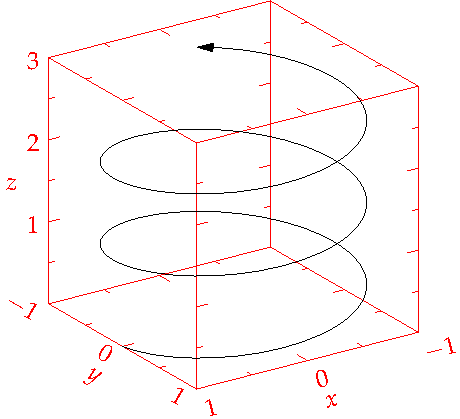
\includegraphics[width=\linewidth]{helix}
  \caption{This is a margin figure.  The helix is defined by 
    $x = \cos(2\pi z)$, $y = \sin(2\pi z)$, and $z = [0, 2.7]$.  The figure was
    drawn using Asymptote (\url{http://asymptote.sf.net/}).}
  \label{fig:marginfig}
\end{marginfigure}

\begin{docspec}
\textbackslash begin\{marginfigure\}\\
  \qquad\textbackslash includegraphics\{helix\}\\
  \qquad\textbackslash caption\{This is a margin figure.\}\\
  \qquad\textbackslash label\{fig:marginfig\}\\
\textbackslash end\{marginfigure\}\\
\end{docspec}

The \docenv{marginfigure} and \docenv{margintable} environments accept an optional parameter \docopt{offset} that adjusts the vertical position of the figure or table.  See the ``\nameref{sec:sidenotes}'' section above for examples.  The specifications are:
\begin{docspec}
  \textbackslash{begin\{marginfigure\}[\docopt{offset}]}\\
  \qquad\ldots\\
  \textbackslash{end\{marginfigure\}}\\
  \mbox{}\\
  \textbackslash{begin\{margintable\}[\docopt{offset}]}\\
  \qquad\ldots\\
  \textbackslash{end\{margintable\}}\\
\end{docspec}

Figure~\ref{fig:fullfig} is an example of the \docenv{figure*}
environment and figure~\ref{fig:textfig} is an example of the normal
\docenv{figure} environment.

\begin{figure*}[h]
  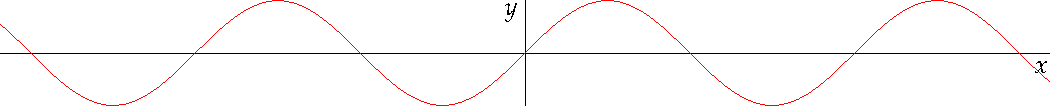
\includegraphics[width=\linewidth]{sine.pdf}%
  \caption{This graph shows $y = \sin x$ from about $x = [-10, 10]$.
  \emph{Notice that this figure takes up the full page width.}}%
  \label{fig:fullfig}%
\end{figure*}

\begin{figure}
  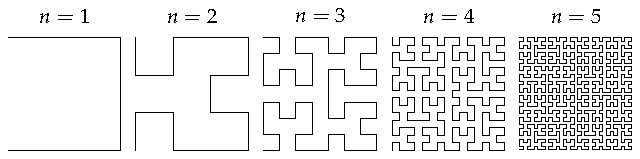
\includegraphics{hilbertcurves.pdf}
%  \checkparity This is an \pageparity\ page.%
  \caption[Hilbert curves of various degrees $n$.][6pt]{Hilbert curves of various degrees $n$. \emph{Notice that this figure only takes up the main textblock width.}}
  \label{fig:textfig}
  %\zsavepos{pos:textfig}
\end{figure}

\chapter{Conclusion}


%%
% The back matter contains appendices, bibliographies, indices, glossaries, etc.







\backmatter

\bibliography{biblio}
\bibliographystyle{apalike}


\printindex

\end{document}

